Bei einem Event entstehen im Detektor Elektron-Loch-Paare, diese driften im angelegten Potential zu den entsprechend geladenen Elektroden.
Die bewegten Ladungen erzeugen einen Signalstrom wie in Abb. \ref{fig:RamoEq} dargestellt.
Das Ersatzschaltbild ist eine zeitabhängige Stromquelle parallel zur Detektorkapazität.
Entgegen der Intuition entsteht der Strom nicht erst, wenn die Ladungsträger die Elektroden erreichen, wie es der Begriff charge collection suggeriert, sondern unmittelbar mit der Entstehung der Ladungsträger.
Das bedeutet insbesondere, dass kein direkter Kontakt der Elektroden mit dem sensitiven Volumen des Detektors notwendig ist.

\begin{figure}[!b]
\begin{center}
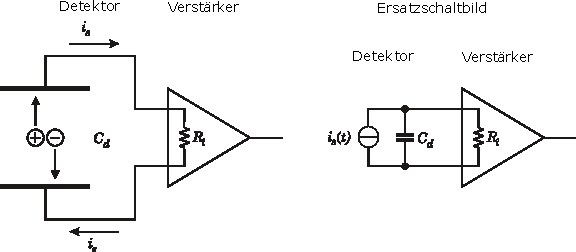
\includegraphics[scale=1.25]{./fig/RamoEquivalent.pdf}
\end{center}
\vspace{-0.5cm}
\caption{Links: Ladungsträger welche sich im Detektorvolumen bewegen erzeugen einen Strom im Schaltkreis. Rechts: Ersatzschaltbild der Schaltung Links. Der Detektor kann als Kapazität mit paralleler, zeitabhängiger Stromquelle dargestellt werden.\cite{Editors}}
\label{fig:RamoEq}
\end{figure}

Für ein qualitatives Verständnis betrachte man eine Ladung $q$, welche sich in der Mitte zwischen zwei unendlich großen Elektroden befindet, wie in der Abbildung \ref{fig:RamoQual} links dargestellt.
Die Hälfte der Feldlinien terminieren auf der oberen und die andere Hälfte auf der unteren Elektrode.
Integriert man nun den Gaußschen Satz über eine Fläche $S_1$ welche die obere Elektrode umschließt oder eine Fläche $S_2$ welche die untere Elektrode umschließt ergibt sich
\begin{equation}
\oint_{S_1} \vec{E} \,d\vec{a} = \oint_{S_2} \vec{E} \,d\vec{a} = -\frac{q}{2}.
\end{equation}
Das heißt auf beiden Elektroden wird die gleiche Ladung von $-q/2$ induziert.
Befindet sich dieselbe Ladung nun in unmittelbarer Nähe zur unteren Elektrode wie in Abb. \ref{fig:RamoQual} rechts dargestellt, terminiert der Großteil der Feldlinien an der unteren Elektrode.
Die induzierte Ladung ist somit in der unteren Elektrode deutlich größer.
Eine Ladung, die sich also von der oberen zur unteren Elektrode bewegt, induziert eine abnehmende Ladung in der oberen Elektrode und eine zunehmende Ladung in der unteren Elektrode.\cite{Editors}

\begin{figure}[!b]
\begin{center}
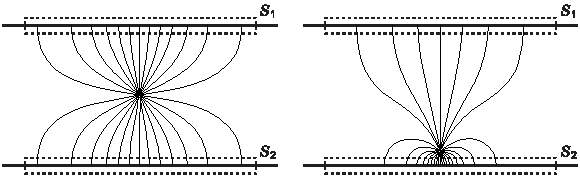
\includegraphics[scale=1.25]{./fig/RamoQual.pdf}
\end{center}
\vspace{-0.5cm}
\caption{Links: Eine Ladung $q$ in der Mitte zwischen zwei Elektroden induziert die gleiche Ladung in beiden Elektroden.
Aus dem Gaußschen Satz folgt, dass die Flächen $S_1$ und $S_2$ jeweils die Ladung $-q/2$ einschließen.
Rechts: Befindet sich die Ladung in der Nähe der unteren Elektrode, terminiert der Großteil der Feldlinien an dieser Elektrode.
Daher ist die Ladung, welche von $S_2$ eingeschlossen ist, größer als die Ladung, welche von $S_1$ eingeschlossen ist. \cite{Editors}}
\label{fig:RamoQual}
\end{figure}

Quantitativ wird dieser Effekt durch das Shockley-Ramo-Theorem beschrieben.
Shockley hat diesen Effekt als erstes im Jahr 1938 beschrieben.
Ramo veröffentlichte allerdings eine deutlich elegantere Formulierung im Jahr 1939.
Der durch eine sich mit der Geschwindigkeit $\vec{v}$ bewegten Ladung $q$ erzeugte instantane Strom ist gegeben durch
\begin{equation}
i_k = -q\vec{v}\vec{E}_Q.
\label{eq:RamoCurrent}
\end{equation}
Das weighting field $\vec{E}_Q$ unterscheidet sich entscheidend vom Elektrischen Feld zwischen den Elektroden.
Während das weighting field den induzierten Strom bestimmt, ist es das elektrische Feld, welches die Dynamik der Ladungsträger beschreibt.
Das weighting field $\vec{E}_Q$ erhält man, indem die Ladung $q$ entfernt wird, die gegebene Elektrode auf das Potential $1$ gesetzt wird und alle anderen Leiter geerdet werden.\cite{Ramo1939}
Die durch eine Ladung $q$, welche sich von $x_1$ zum Zeitpunkt $t_1$ nach $x_2$ zum Zeitpunkt $t_2$ bewegt, induzierte Ladung ergibt sich aus der Integration des Stroms $i_k$ über die Zeit
\begin{align}
\Delta Q_k &= \int_{t_1}^{t_2}i_k \,dt = \frac{1}{|\vec{v}|} \int_{\vec{r}_1}^{\vec{r}_2}i_k \,dr = -\frac{q}{|\vec{v}|} \int_{\vec{r}_1}^{\vec{r}_2}\vec{v}\vec{E}_Q \,dr = \frac{q}{|\vec{v}|} \int_{\vec{r}_1}^{\vec{r}_2}\vec{v}\nabla\Phi \,dr \nonumber \\
&= q\left(\Phi(r_2) - \Phi(r_1)\right).
\label{eq:RamoCharge}
\end{align}
Das weighting potential $\Phi$ hängt über $\vec{E}_Q = -\nabla\Phi$ mit dem weighting field zusammen.
Die Induzierte Ladung $\Delta Q$ ist unabhängig vom zurückgelegten Weg der Ladung $q$.
Sie ist ausschließlich abhängig vom Anfangs- und Endpunkt.

In Abbildung \ref{fig:RamoDeLight} ist der Fall zweier von einem Kristall vakuumseparierten Elektroden dargestellt.
Die Ladungsträger driften nur innerhalb des Kristalls.
Zwischen Elektrode und Kristall fällt bereits ein Teil des Potentials ab.
Daher durchlaufen die Ladungsträger im Kristall nur einen Teil des angelegten Potentials.
Um die induzierte Ladung entsprechend dem Ramo-Theorem zu berechnen wird das \textit{weighting potential} $\Phi$ bestimmt
\begin{align*}
\Phi(d) &= 1 \\
\Phi(h+g) &= a\\
\Phi(g) &= b\\
\Phi(0) &= 0.
\end{align*}
Ein Event im Detektorvolumen erzeugt eine bestimmte Anzahl von Elektron-Loch-Paaren $N_{eh}$ in der Höhe $z_0$.
Angenommen das Potential $V_0$ ist positiv, dann driften die Elektronen in Richtung der 
Elektrode $A$ und die Löcher in Richtung der Elektrode $B$.
Für die auf der Elektrode $A$ induzierte Ladung $\Delta Q$ ergibt sich somit nach Gleichung \eqref{eq:RamoCharge}
\begin{align}
\Delta Q &= e N_{eh}(\Phi(g) - \Phi(z_0)) + (-e)N_{eh}(\Phi(h+g) - \Phi(z_0)) \nonumber \\
&= eN_{eh}\left(b - \Phi(z_0) - a + \Phi(z_0)\right) \nonumber \\
&= -eN_{eh}(a-b).
\label{eq:RamoCharge}
\end{align}
Diese ist unabhängig von der genauen Position $z_0$ des Events.
$(a-b)$ gibt den von den Ladungsträgern durchlaufenen Prozentteil des gesamten Potentials an.
Entsprechend wird auf der Elektrode $B$ die Ladung $\Delta Q = eN_{eh}(a-b)$ induziert.


\begin{figure}[!t]
\begin{center}
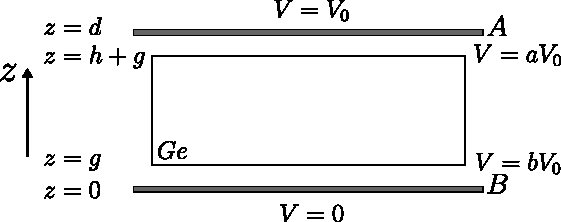
\includegraphics[scale=1.25]{./fig/ElektrodenDeLight.pdf}
\end{center}
\vspace{-0.5cm}
\caption{Verlauf des Potentials in z-Richtung für einen Kristall zwischen zwei vakuumseparierten Elektroden A und B.
Annahme eines Homogenen Feldes in x- und y-Richtung. 
Zwischen Elektrode und Ge-Kristall fällt das Potential von $V_0$ auf $aV_0$ und von $bV_0$ auf $0$ ab, mit $0 < b < a < 1$.}
\label{fig:RamoDeLight}
\end{figure}